\chapter{Paper 1}

The differential equation can be non-dimensionalized by letting $\tau$ and $y(\tau)$ be the non-dimensional quantities, and letting $C(t) = k_a FD/V y(\tau)$ and $t = \tau/k_a$.  The non-dimensionalized differential equation is then

\begin{equation}
	\dfrac{dy(\tau)}{d\tau} = \exp(-\tau) - \alpha y(\tau)
\end{equation}

\noindent Here, $\alpha = k_e / k_a$ is the ratio of elimination and absorption rates, and is dimensionless.  The differential equation's qualitative behaviour depends solely on this ratio, with all parameterizations in which $\alpha$ is constant displaying the same qualitative behaviour.  The remaining variables $V$, $D$, and $F$ only serve to scale the solution vertically.  The solution to this differential equation (obtained via integrating factors or the Laplace Transform) is

\begin{equation}\label{key}
	y(\tau) = \dfrac{1}{\alpha -1} \Big( \exp(-\tau) - \exp(-\alpha \tau) \Big)
\end{equation}

\noindent which can be transformed back into dimensional variables to yield 

\begin{equation}\label{onecompartment_PKPD}
	C(t) = \dfrac{F D}{V}\dfrac{k_a}{k_e - k_a}\Big(e^{-k_at} - e^{-k_et}\Big) \>.
\end{equation}

\begin{figure}[h!]
	\centering
	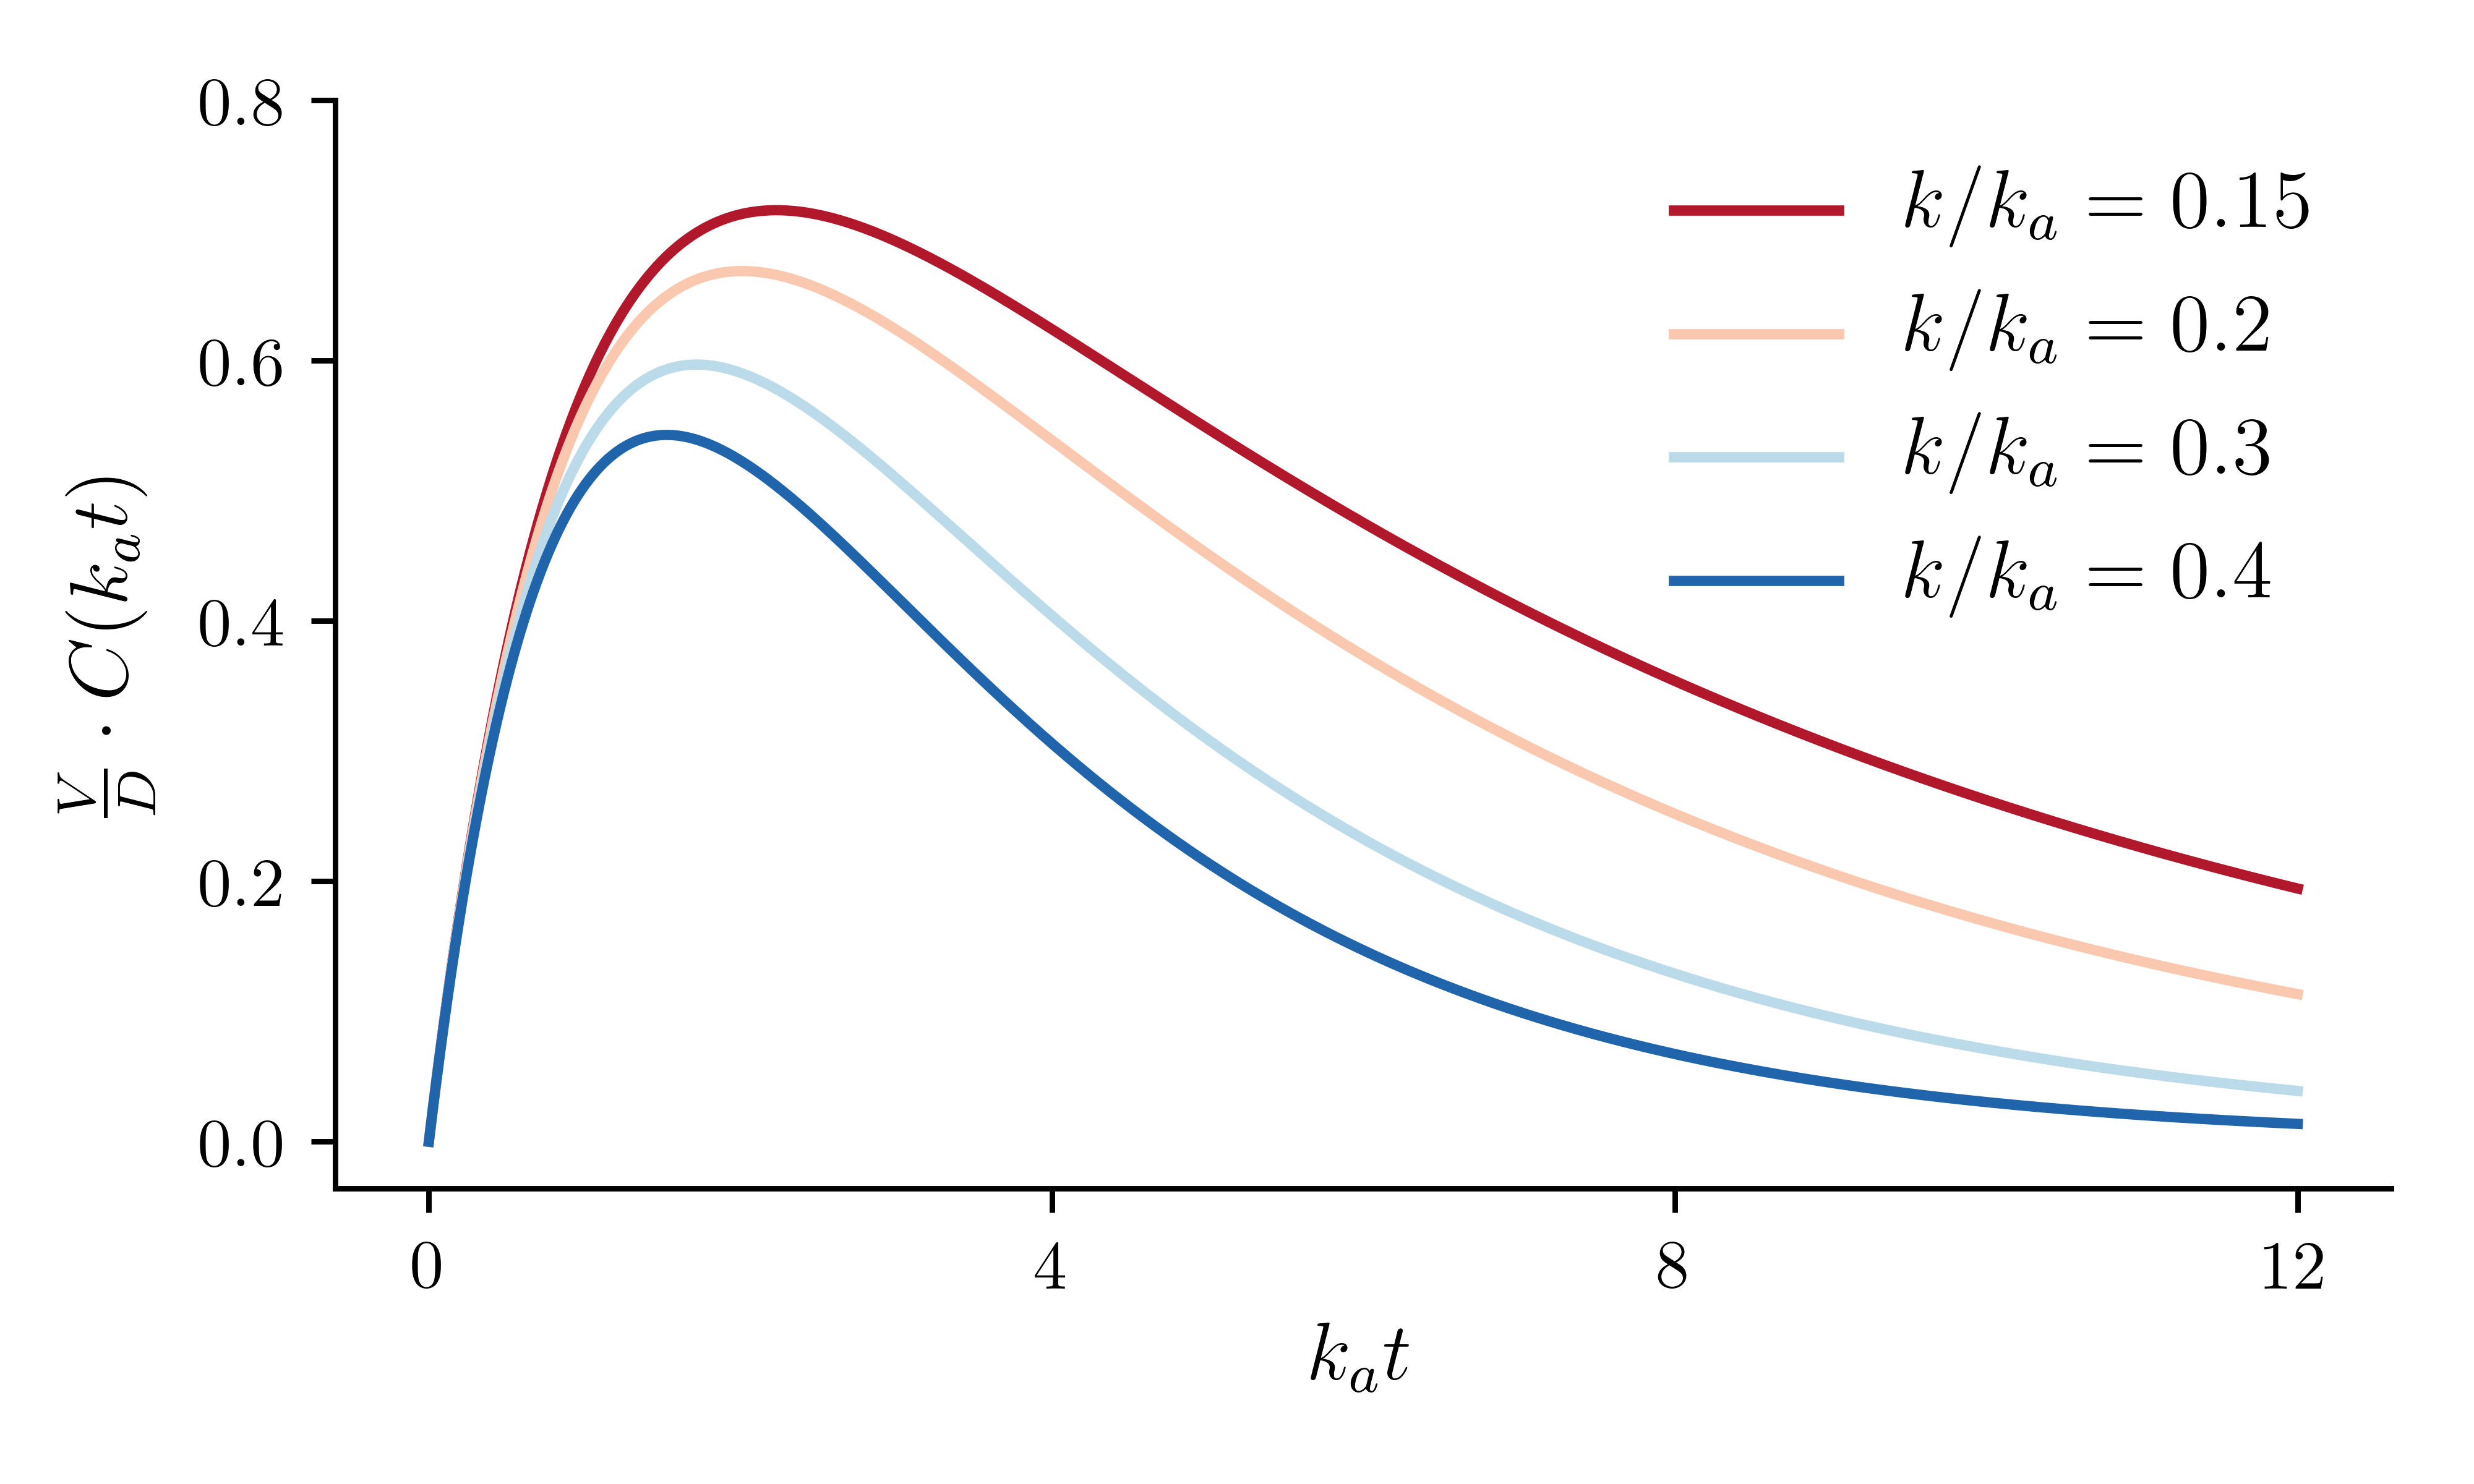
\includegraphics{figures/pkcurves.png}
	\caption[Non-dimensionalized solutions to pharmacokinetic differential equation] {Non-dimensionalized concentration plotted against non-dimensionalized time.  The process non-dimensionalizing the differential equation removes all units from the model, allowing for qualitative comparisons of the solution under different families of parameterization.  Here, it is shown that all parametrizations in which $\alpha = k_e/ka = 0.15$ elicit larger concentrations than those parameterizations in which $\alpha=0.4$ conditioned on $FD/V$ remaining constant.}
	\label{fig:pkcureves}
\end{figure}



\section{Introduction}

Precision medicine’s slogan is ``right drug -- right patient -- right time''.  Implicit in the slogan is ``right dose''; however, determining the right dose for any one patient can be challenging. The anticoagulant Warfarin offers a good example of these challenges; physicians choose an initial dose based on guidelines and their own experience. They then closely monitor the patient’s International Normalised Ratio (INR), which measures how long it takes blood to clot, and in response they adjust the dose over time.

Pharmacokinetic and statistical models of how drugs behave within an individual can alleviate some of these challenges by predicting the effects of different doses based on patient covariates. In some studies \cite{schwarz2008genetic,Sohrabi2017-zv, Caldwell2007-mi}  a cohort of patients will have an appropriate maintenance doses determined empirically and these are then regressed onto patient covariates.  In others \cite{ohara2019differences,Zhu2017-rk, Xue2017-mp}  patient pharmacokinetics are directly modeled and can be simulated under different dosing regimens to find an appropriate dose.  In both cases, uncertainty in the models can be assessed and can help guide clinical decisions as to what dose is best or what dose to try next.

Both types of  models can provide guidance for individual patients, but only when there is enough data so that the models are accurate and reliable. For personalized pharmacokinetics-based dosing, this amount of data is rarely available in practice.  Obtaining sufficient data to learn a patient’s pharmacokinetic parameters requires a lengthy observation period which few patients are willing or capable of committing to. Population pharmacokinetic models could be used in place of a patient’s pharmacokinetics, but treating the patient as “average” is precisely what precision medicine seeks to improve upon.

In many contexts where limited data area available, Bayesian methods with informative priors have been proposed.  Model priors allow analysts to specify their beliefs about model parameters prior to seeing a new patient's data, and to combine those beliefs with new observations to form personalized predictive models.  This allows models to ``hit the ground running'' so to speak, and makes use of all available data to support decision-making.  To use all but the simplest of Bayesian models for decision-making requires computational approximation techniques to obtain model estimates and predictions. Several approaches exist for generating approximate samples from the posterior distribution, with Hamiltonian Monte Carlo (HMC) being considered the gold standard \cite{Neal1996-vn, Matthew_D_Hoffman2014-in, Carpenter2017-qf, Tripuraneni2017-oh}. Despite HMC being the preferred method by theorists and applied Bayesians alike, methods like Maximum A Posteriori (MAP), in which the posterior mode is computed via optimization and then a Laplace approximation is performed, continue to be used in population Bayesian pharmacokinetic studies as late as 2020 \cite{Brooks2016-li, Nguyen2016-pg,  Preijers2019-kc,Stifft2020-uq}. HMC and MAP are two different approaches with different strengths and different theoretical motivations. Naturally, this raises questions regarding how decisions in personalized medicine may be affected by the use of different methods for performing inference, even using the same model and data. We seek to answer these questions by developing a new, high-fidelity Bayesian pharmacokinetic model and then investigating the impact of the choice of inference method on precision medicine decisions. 

\subsection*{Generalizable Insights about Machine Learning in the Context of Healthcare}

The main methodological insight we gained was that \textit{although predictions made by HMC and MAP may appear to be very similar according to common error metrics, they can lead to very different personalized dosing decisions.} The main contributions of this paper are as follows: 

\begin{enumerate}
\item A new Bayesian model for apixaban pharmacokinetics written in an open source Bayesian language.  We make the model code and posterior summaries of all parameters publicly available at https://github.com/Dpananos/PKBayes.

\item A simulation study demonstrating that inferences made via MAP and HMC lead to very different dosing strategies.

\item An induction dosing model for apixaban based on desired trough concentration level after a first dose.
\end{enumerate}




